\section{Cronograma de las actividades realizadas}

Inicialmente realizamos un cronograma tentativo en forma de diagrama de Gantt de la totalidad del trabajo, incluyendo el desarrollo de cada caso de uso, el despliegue en cada ecosistema y su documentación asociada como se muestra en la Figura \ref{fig:cronograma-tentativo}. Sin embargo, a medida que fuimos desarrollando el trabajo nos encontramos con que dividir el trabajo por ecosistemas era más eficiente que dividirlo por casos de usos como en nuestro cronograma estimado.

\begin{figure}[H]
    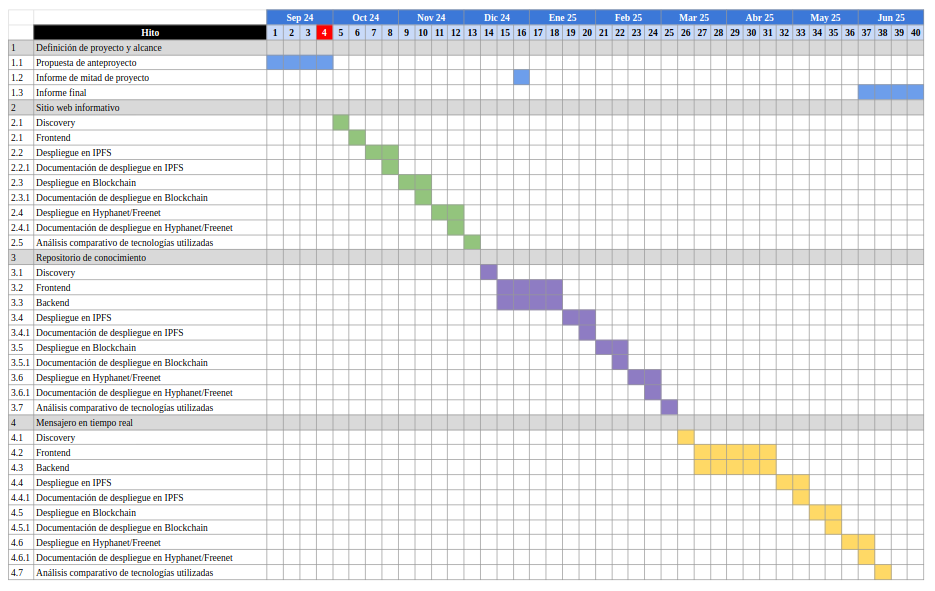
\includegraphics[width=1\linewidth]{img/cronograma.png}
    \caption{Cronograma tentativo}
    \label{fig:cronograma-tentativo}
\end{figure}

Por lo tanto, lo que terminó sucediendo es lo que se muestra en la Figura \ref{fig:cronograma-real}. La división se hizo por ecosistema, esto incluye la investigación, el desarrollo y la documentación de cada caso de uso para el ecosistema en cuestión. Hacerlo de esta manera nos permitió paralelizar los esfuerzos y evitamos superposiciones durante la investigación y desarrollo. Esta separación podría haber generado silos de conocimiento por ecosistema dentro del equipo, es por esto que las reuniones semanales de puesta en común, junto con la constante comunicación por chat y sesiones de \textit{pair-programming}, fueron de vital importancia para mitigar dicha separación y que todo el equipo esté al tanto de los conocimientos adquiridos de cada ecosistema.

\begin{figure}[H]
    \centering
    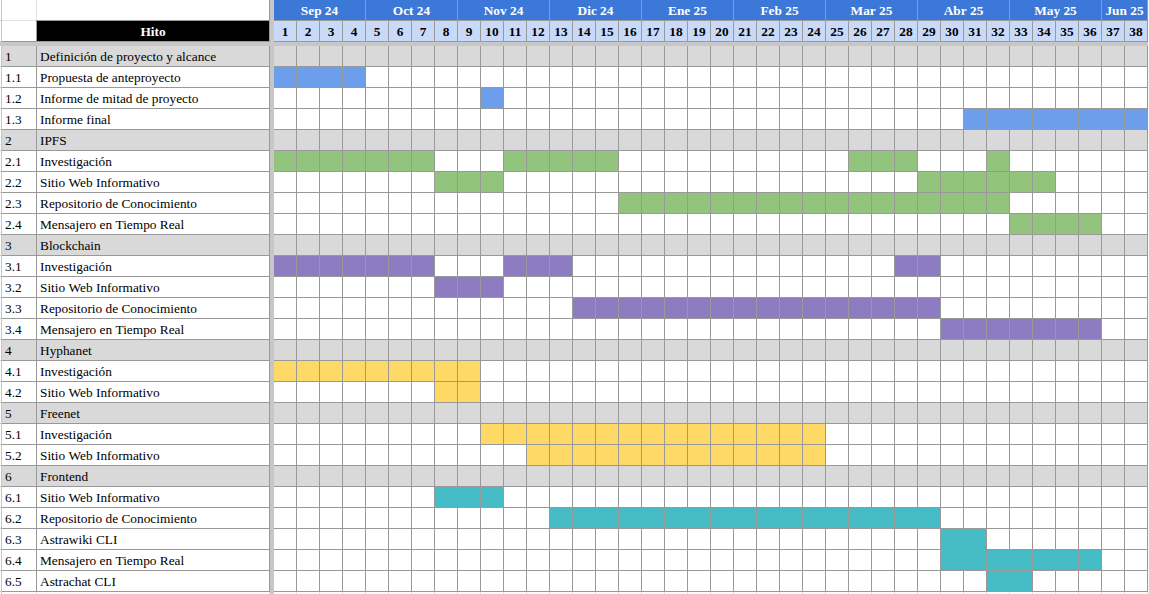
\includegraphics[width=1\linewidth]{img/cronograma-real.png}
    \caption{Cronograma real}
    \label{fig:cronograma-real}
\end{figure}

En el cronograma real se puede ver que el desarrollo del repositorio de conocimiento en IPFS llevó más tiempo a comparación del mensajero en tiempo real. Esto fue debido a que, a medida que se fue desarrollando el repositorio de conocimiento, se fueron realizando abstracciones (como la separación en packages y AstraDB) que permitieron que el desarrollo del mensajero en tiempo real sea más sencillo y lleve menos tiempo. Algo similar sucedió para blockchain, donde notamos que los contratos para ambos casos de uso resultaron ser bastantes similares.

Además, antes del desarrollo de cada caso de uso dedicamos un tiempo a la investigación en cada ecosistema, esto incluyó: análisis de herramientas existentes, confección de \textit{User Story Mappings} y lectura de documentación de cada ecosistema.

Por último, podemos notar el momento justo en el que dejamos de realizar el desarrollo de Hyphanet y Freenet, que fue en donde entró en juego nuestro plan de contingencia. 